The web frontend is designed to provide an intuitive exploration of the different datasets, clustering algorithms and distances. In an interactive interface multiple clustering settings can be chosen and a visualisation of the results is directly generated. 
A cluster-table is used to store previous calculated results, which can be plotted within the evaluation module. \\
A checkbox at the top of the page (see \autoref{fig:parameters} A), which is set by default, allows the use of precalculated clustering results, which have been computed beforehand (with a random seed value) and are stored in the github repository. This was done for reproduction purposes. The second checkbock (see \autoref{fig:parameters} B) allows the option for interactive projection plots.  \\
The user can choose between four datasets (see \autoref{fig:parameters} C), four distance measures (see \autoref{fig:parameters} E) and four different algorithms (see \autoref{fig:parameters} D). If kmeans, kmedian or kmedoids is chosen a value for the parameter k between 1 and 10 has to be set (see \autoref{fig:parameters} F) The default value for k is 3. If DBSCAN is chosen the user has to define a value for epsilon and the minimal number of nearest points. The parameter settings can be adjusted with an interactive slider widget. \\
\begin{figure}[H]
	\centering
	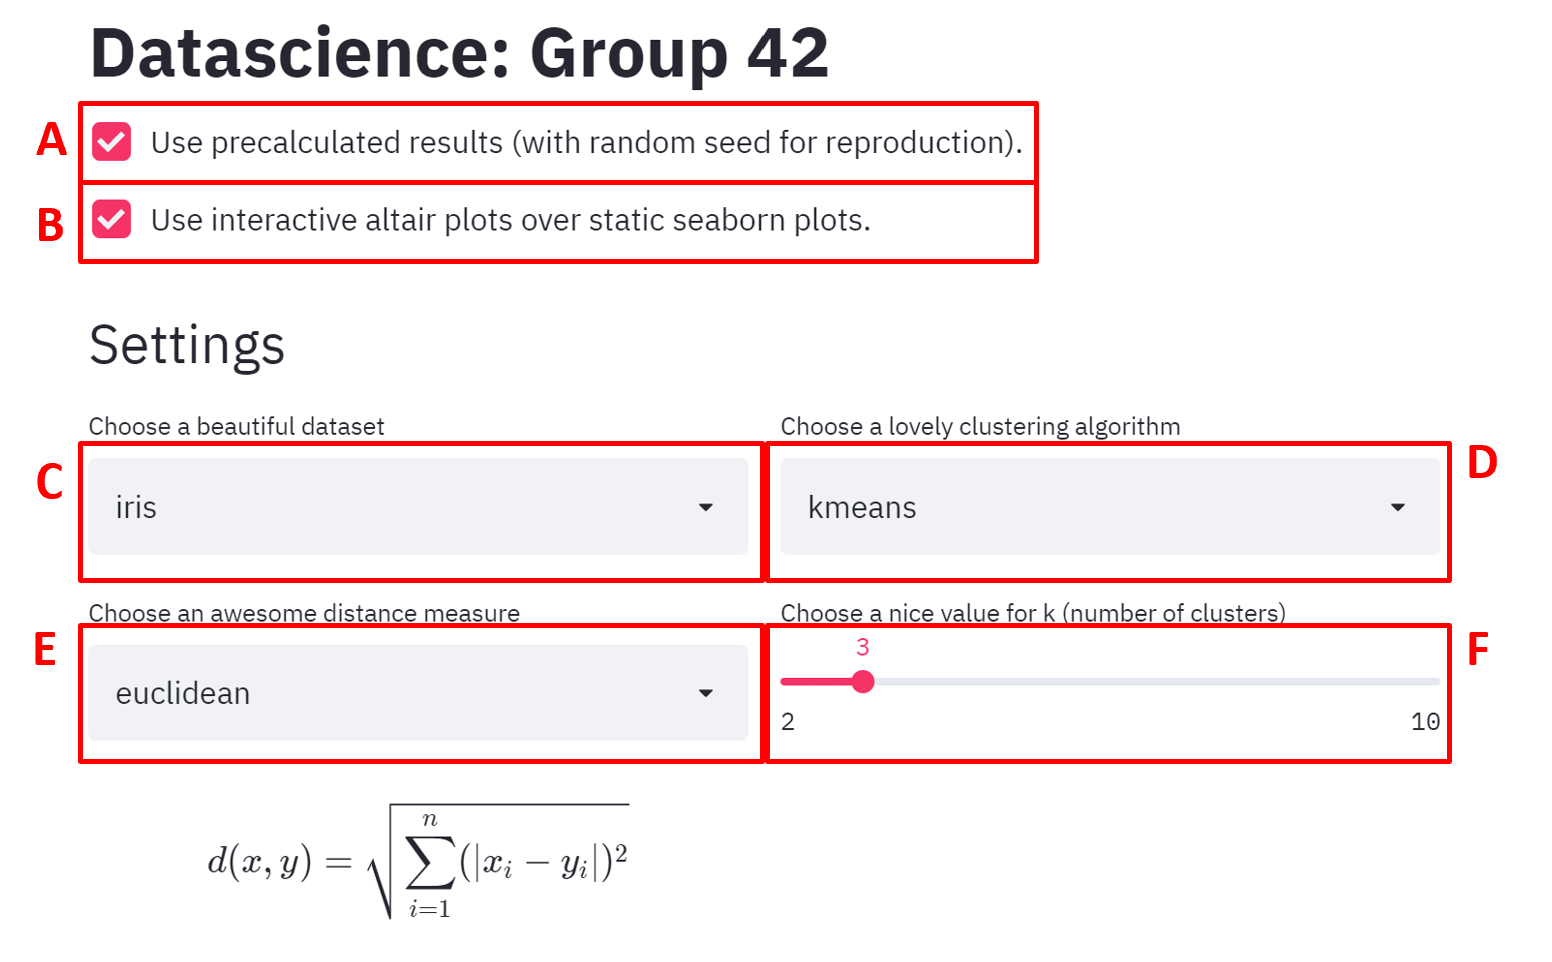
\includegraphics[width=\linewidth]{modules/web_frontend/eingabe_letters}
	\caption{First part of the web frontend. Setting options for clustering parameters.}\label{fig:parameters}
\end{figure}

Moreover the perplexity value for the t-SNE projection can be set individually between 5 and 50 with a slider (see \autoref{fig:projection} A). The default value is 25. The t-SNE and PCA plots are shown next to each other to allow a direct comparison of the lower-dimensional projections. To virtually interact with the plots, the button shown in \autoref{fig:projection} C can be clicked. Please note that this option is only available when the checkmark shown in \autoref{fig:parameters} B is set. Furthermore, this button provides the ability to save the plot in different formats.
The selected dataset can be viewed in a table format below the plots (see \autoref{fig:projection} B).
The frontend is reloaded entirely if a parameter value is changed, a different setting is made or a button is clicked. 
\begin{figure}[H]
	\centering
	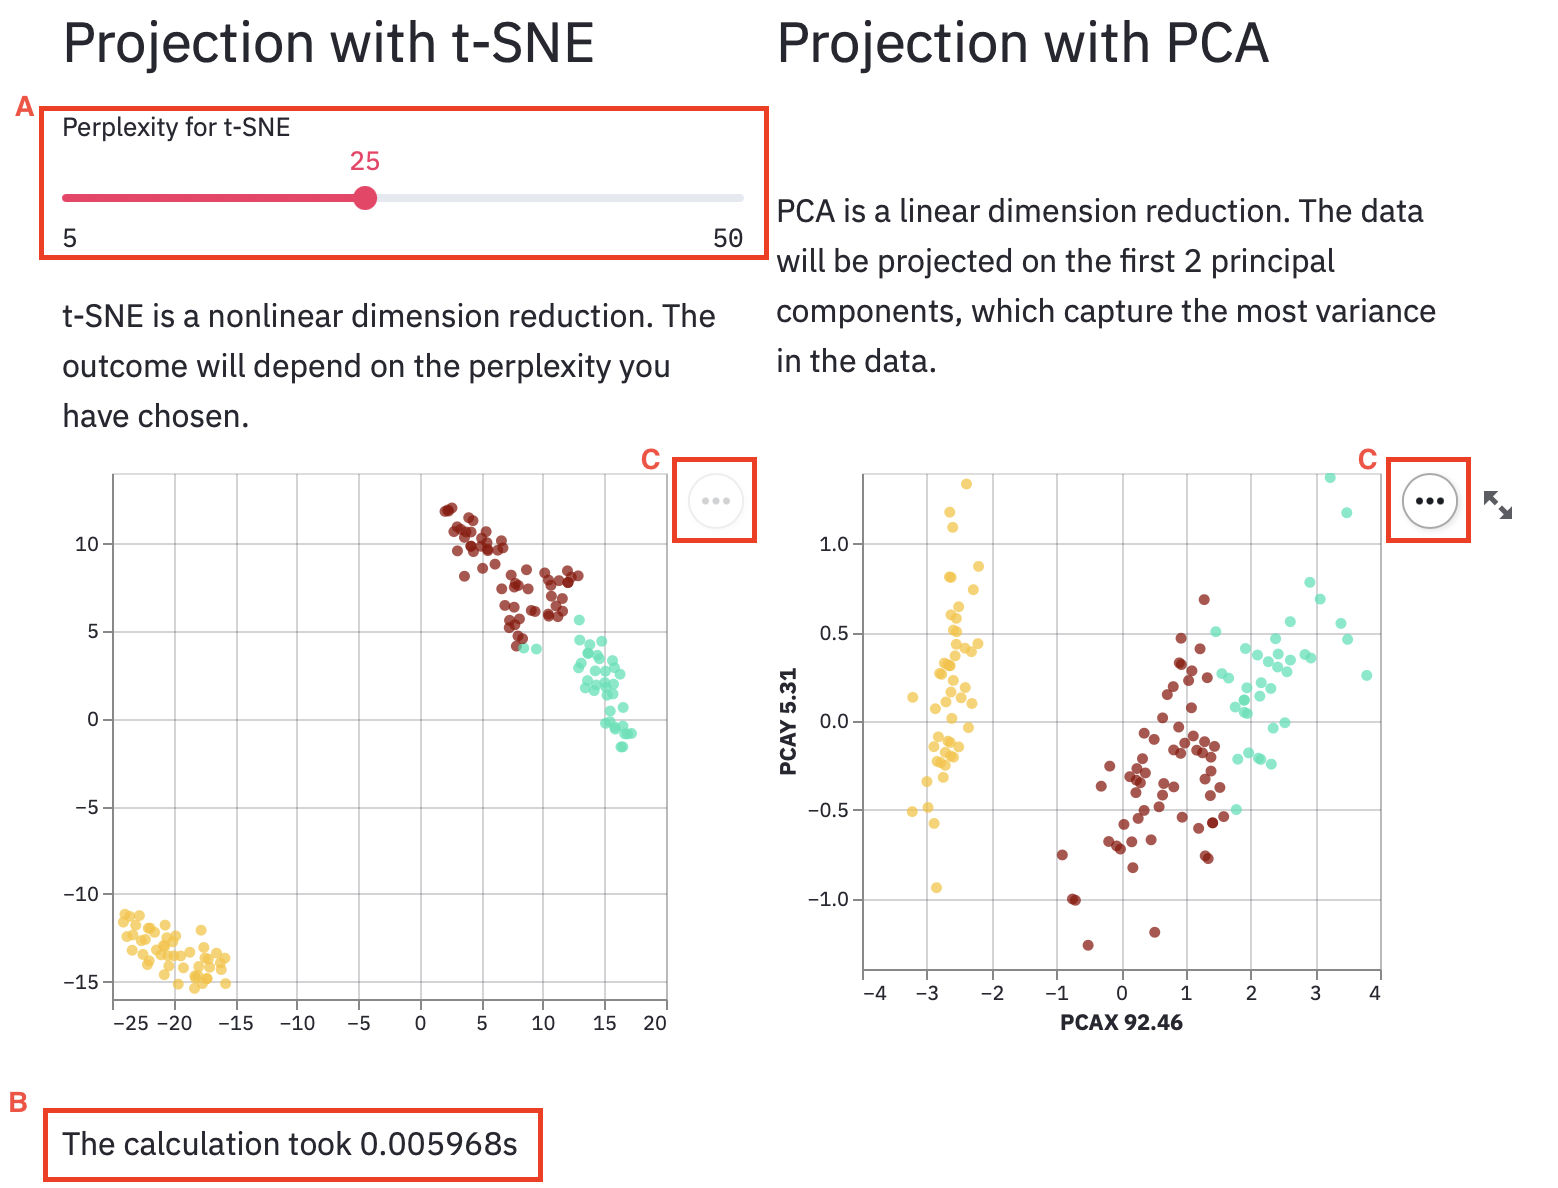
\includegraphics[width=\linewidth]{modules/web_frontend/projection_letters}
	\caption{Second part of the web frontend. Projection results of a clustering.}\label{fig:projection}
\end{figure}

For the evaluation of the clustering results, a clustering index can be chosen as shown in \autoref{fig:evaluation} C. Afterwards, the clustering result can be saved through addition to the clustering table with the \textit{add}-button (see \autoref{fig:evaluation} A) and the selected index will be calculated. To compare this index to the resulting indices of clusterings with other settings, the \textit{add}-button can be clicked repeatedly after desired adjustment of the clustering settings. To start over and compare further clustering indices, the \textit{reset}-button (see \autoref{fig:evaluation} B) can be clicked. The previous display of resulting indices will be cleared as well as the clustering table. 
\begin{figure}[H]
	\centering
	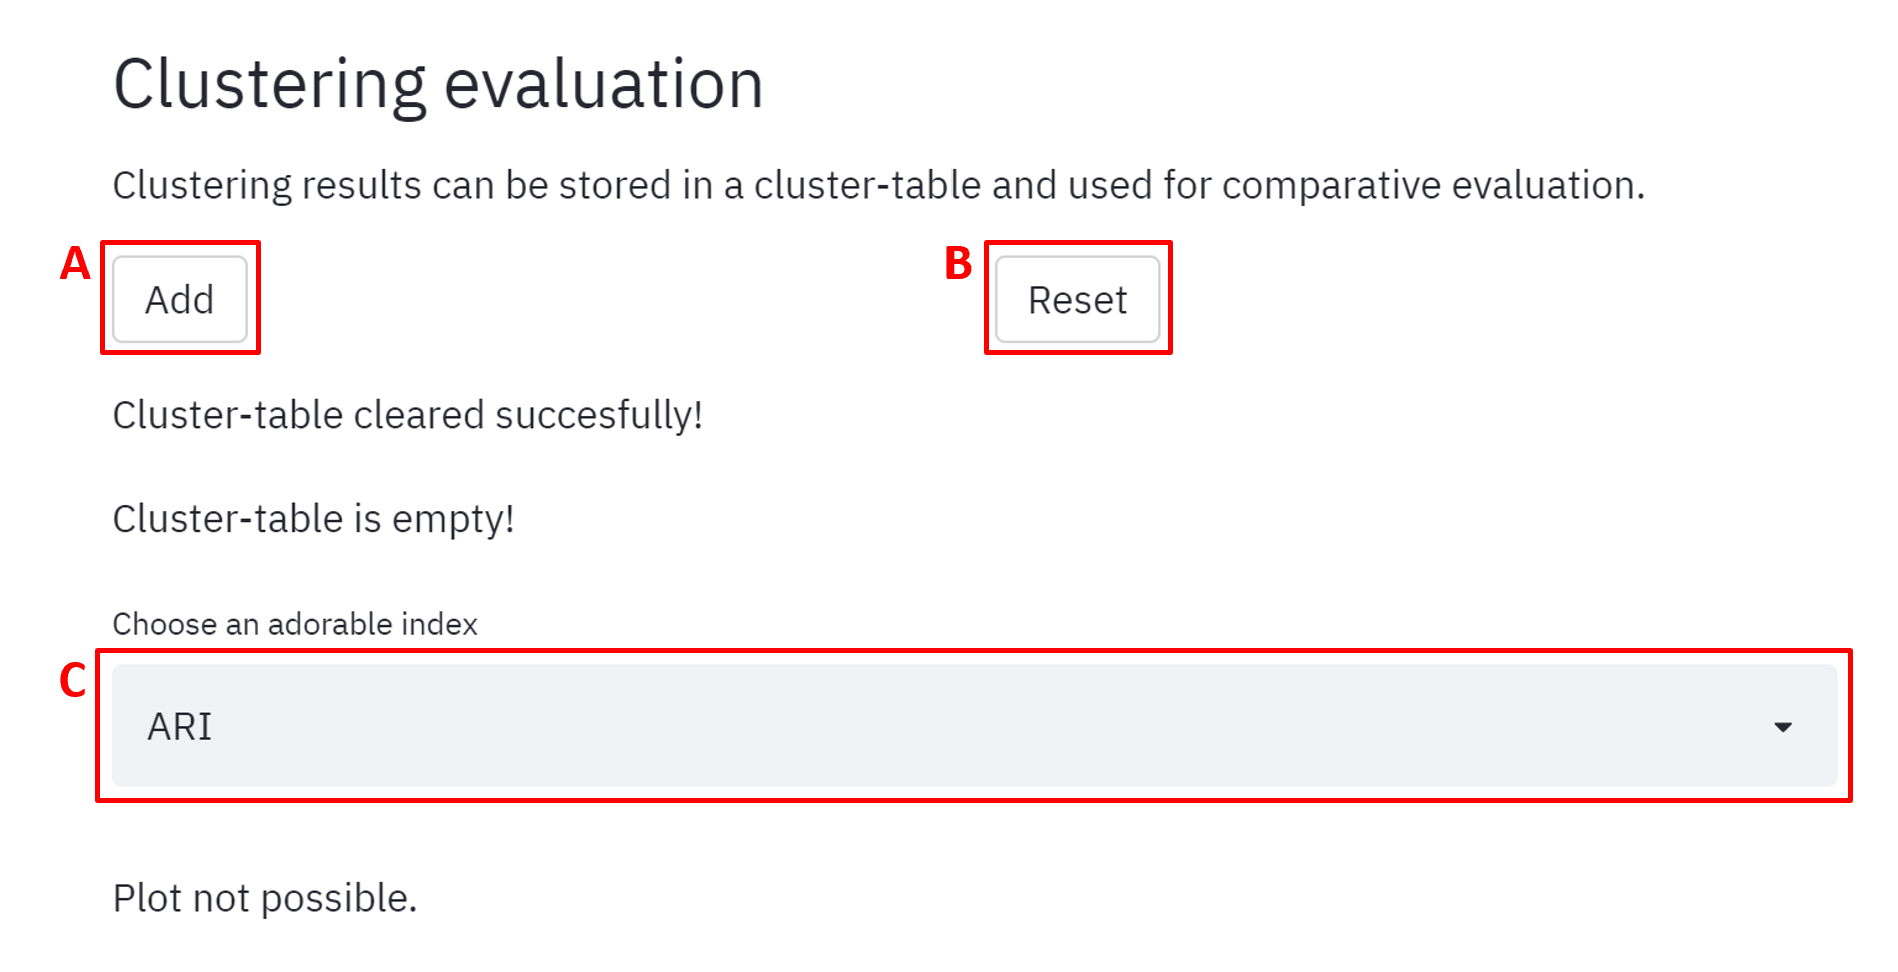
\includegraphics[width=\linewidth]{modules/web_frontend/evaluation_letters}
	\caption{Third part of the web frontend. Evaluation of clustering results.}\label{fig:evaluation}
\end{figure}


Ancillary streamlit settings can be found at the upper right corner. Additional explanatory texts provide help and more information. \\
To motivate the user and claim serious scientific standards some ballons have been added. 
